\section{Designing a compiler for fluxional compliancy} \label{section:compiler}

% The section \ref{section:model} of this paper describes the fluxional execution model, a framework to run web application in a distributed environment.
% This section explains the compiler we developed to transform a subset of classic web application to be compliant with the execution model previously described.
% This transformation unveils two problems due to the differences between a web application and the execution model.
% In the first section, a distributed system is defined by the parallel execution of its parts, and the distribution of its memory.
Current Web applications are mostly written in Java. The langage proposes both data encapsulation and a threading model that ease the development of distributed applications.
Yet, Java framework for developing efficient applications are complex systems that impose new APIs\cite{Coward2003} to the developers.
They are error-prone, and leads to deadlocks and other synchronization problems.
Since 2009, \textit{Node.js}\cite{Dahl} provides a Javascript execution environnment for network applications.
We focus on this promising environment for its initial simplicity and efficiency.
We develop a compiler that transforms a \textit{Node.js} application into a fluxional system compliant with the architecture described in section \ref{section:model}.
As javascript forbids user-space thread API, a javascript application is developed as a mono-threaded application.
Moreover, in Javascript  the memory is hierarchical and the root scope may be accessed by any function, which leads to bad component isolation.
Our compiler uses a new approach to find rupture points marking out independent parts into most of \textit{Node.js} applications.
It assures isolation and memory consistency for the application parts.

We do not target all Javascript Web-based application as this work is only a proof of concept for the compilation.
If we are able to transform a consequent subset of currently running applications without external developer help, we expect a real execution gain in a cloud environment.
The rest of this section describes the two parts of the compiler responsible to isolate application parts.
Section \ref{section:analyzer} explains how the \textit{analyzer} detects rupture points in the web application to mark out the independent parts.
Section \ref{section:linker} explains how the \textit{linker} resolves the missing dependencies due to the distribution of the central memory.

% TODO move this
% The compiler reuses some tools from the Javascript community.
% The compiler and these tools follow the specification for an intermediate representation of the Javascript source code from the Mozilla Javascript Parser API\cite{JsAST}.
% \textit{Esprima}\cite{esprima} parses the source and generate an Abstract Syntax Tree (AST).
% The compiler analyze and modify this tree by traversing it using \textit{Estraverse}\cite{estraverse}.
% \textit{Escope}\cite{escope} extracts function scopes and variables declaration from the tree.
% At the end of the compilation chain, the compiler uses \textit{Escodegen}\cite{escodegen} to transform AST back into Javascript source code.

\subsection{Analyzer : execution parallelism} \label{section:analyzer}

% The parallelization of programs is a trending problem to leverage the multiple cores available on highly parallel architectures.
The Sun programming guide\footnote{\raggedright http://docs.oracle.com/cd/E19455-01/806-5257/6je9h032b/index.html} defines \textbf{parallelism} as \textit{a condition that arises when at least two threads are executing simultaneously}, and \textbf{concurrency} as \textit{a condition that exists when at least two threads are making progress. A more generalized form of parallelism that can include time-slicing as a form of virtual parallelism}.
\textbf{Asynchronism} is a condition that arises when a client continues its execution while waiting for the result to its request.

% When the result of the asynchronous request is available for the client, a synchronization mechanism is used to retrieve it.
% Examples of synchronization methods are Promises\cite{Liskov1988} or callbacks.
% A callback uses the pattern of inversion of control.
% Instead of the client waiting for the result, the system calls back the client with the available result.

% The caller of the asynchronous operation can continue its execution until the end.
% The callee of the asynchronous operation is executed in parallel with the caller, in a dedicated thread of execution.
% When the callee finishes, the result of the execution is available.

% The caller and the callee are not executed in the same thread of execution.
% But the continuation of execution after the callee is executed in the same thread as the callback.


% The client doesn't wait for the result to be available and continue its execution.
% The result is queued to be processed later by the client.
% The client is continuously in execution. At the end of any execution, it dequeues a result from an asynchronous operation to process with a callback.

% The client dequeue the results to execute them on a single thread, while the asynchronous operation happens on parallel threads.
% An asynchronous operation with callback is executed from the main thread, from the asynchronous operation, to the parallel I/O thread, and then to the main thread again.
% But provided with the correct memory isolation, callback could be executed on another thread.
% They contain both the input data, and the processing function in a single object enqueued.
% This model is exactly similar to the pattern thread-pool pattern where all tasks are enqueued on a queue, and dequeued by a pool of thread.

% Node.js uses only one thread to dequeue and execute the callbacks to avoid concurrency in the execution, and the synchronization with it.



% A rupture point is the point where the decision for the callback to be executed on the main thread, or in another thread.
% A rupture point happens between the end of execution of the asynchronous operation and the queuing of the callback.
% A rupture point happens before the callback is queued to be executed.
% A rupture point happens before the choice of the queue onto which enqueue the callback is made.

% A rupture point is the interface between the end of the asynchronous operation and the callback.




% A rupture point is a discontinuity in the execution due to an asynchronous operation.



In the \textit{Node.js} environment, all of the application execution take place in a single thread : the main thread.
When the application calls an asynchronous function, the requested operation takes place in a thread in parallel : the I/O thread.
At the end of this operation, the I/O thread pushes the result and a function to process it in a queue to be executed by the main thread.
This function is named a callback and is provided by the application purposely to process the result of the asynchronous operation.
The \textit{Node.js} environment confine the application to run in a single thread to avoid concurrency and the memory synchronizations problems associated with it.
Without these memory concerns, the callback and the associated result could be deported on a different thread, provided that the needed memory be accessible.

% Promises\cite{Liskov1988} and callbacks, are abstractions that transform blocking synchronous operations into non-blocking asynchronous operations.
% Asynchronous operations run in a thread in parallel with the main, and only, thread of the application ; they don't block the application.
% When the asynchronous operation completes, the requested result is available for the application to retrieve it.
% The asynchronous operation splits the execution in two concurrent execution paths, one that needs the requested result, the callback or the promise, and one that doesn't.
% These two concurrent paths are executed by the main thread of the application.
% A rupture points is where the execution forks in two concurrent paths.
% These points mark out the limits between the independent parts of an application.
 
% The analyzer detects rupture points to break the application into independent parts.
% In this section, we define what a rupture point is, and how the compiler detects them.

\subsubsection{Rupture points}

A rupture point is the discontinuity between the asynchronous operation and the callback execution.
It marks out the separation between two independent application parts, each with a different execution path.
In the \textit{Node.js} environment, these two application parts are executed one after the other on the same execution thread.
But the rupture point split the two application parts and reveal a pipeline parallelism, as defined in\cite{Gordon2006}.
% Rupture points represent a concurrency between two execution paths.
% They are composed of an asynchronous function, and a callback to process the result of the operation.
% The first execution path is the suite of instructions following after the asynchronous function.
% The second execution path is the callback.
% A rupture point is an interface between these two execution paths and splits them in two application parts.
Listing \ref{lst:hello} is an example of a rupture point in a simple application.
The division of this application into two application parts is illustrated figure \ref{fig:flux-1}.
The asynchronous function call \texttt{fs.readFile} and the callback \texttt{function display} represent the rupture point between the first execution path, line \ref{lst:first_ep} and the second, line \ref{lst:second_ep}.
The first application part is the whole program minus the \texttt{function display}, the second application part contains only the \texttt{function display}, lines \ref{lst:callback_begin} to \ref{lst:callback_end}.

\begin{code}[js, caption={Example of a rupture point : an asynchronous function call, \texttt{fs.readFile()}, with a callback parameter, \texttt{function display}},label={lst:hello}]
var fs = require('fs');

@\label{lst:callback_begin}@fs.readFile(__filename, function display(err, data) {
@\label{lst:second_ep}@  console.log('>> second concurrent execution path');
  console.log(err || data.toString());
@\label{lst:callback_end}@})

@\label{lst:first_ep}@console.log('>> first concurrent execution path');
\end{code}

\begin{figure}[h!]
\begin{center}
  
\includegraphics[width=\linewidth]{ressources/flux-1.pdf}
  \caption{Division of the listing \ref{lst:hello} into two application parts, the asynchronous call to \texttt{readFile} and the callback \texttt{function display}}
  \label{fig:flux-1}
\end{center}
\end{figure}

There are two types of rupture points : \textit{start} and \textit{post}.
Figure \ref{fig:basicrp} and \ref{fig:specialrp} illustrate the different interfaces implied by rupture points between two application parts.
In these figures, the two concurrent execution paths are indicated by \circled{1} and \circled{2}, the applications parts are encapsulated in upstream and downstream fluxions.

\textbf{Start rupture points} are on the border between the application and the outside, continuously receiving incoming user requests, like \texttt{app.get()} in listing \ref{lst:rupturepoints}.
These functions indicate the input of a data stream in the program, and the beginning of a chain of application parts following this stream.
% The \textit{start} rupture points will later be used to monitor the load from incoming external requests.
The asynchronous function is called only once, while the callback is triggered for each new request.
The interface of this rupture point is placed between the two, as illustrated in figure \ref{fig:basicrp}, because it implies the least modifications on the program structure.

\textbf{Post rupture points} represent a continuity in the execution flow after a finite asynchronous operation, such as reading a file in listing \ref{lst:hello}.
As the result of this read operation probably is a voluminous object between two application parts, this interface is specially placed before the call to the asynchronous function, but after the resolution of the arguments.
This placement allow the asynchronous function call to occur in the same application parts as the callback, avoiding the transfer of this voluminous result, as illustrated in figure \ref{fig:specialrp}.
% The function calls from following rupture points mark the interface between the current application part and the next one.
For a write operation, the data transfer is the opposite so the interface is placed between the asynchronous operation and the callback, like for a \textit{start rupture point}, as illustrated in figure \ref{fig:basicrp}

The impact of these rupture points on the application structure during the compilation is illustrated in listing \ref{lst:ex-jsres} and explained in section \ref{section:example}.

\begin{figure}[h!]
\begin{center}
  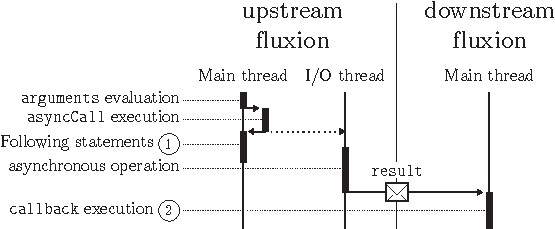
\includegraphics[width=\linewidth]{ressources/basicrp.pdf}
  \caption{Basic rupture point interface. \textnormal{The rupture point interface is placed between the asynchronous operation and the callback to reduce the impact on the application structure.}}
  \label{fig:basicrp}
\end{center}
\end{figure}

\begin{figure}[h!]
\begin{center}
  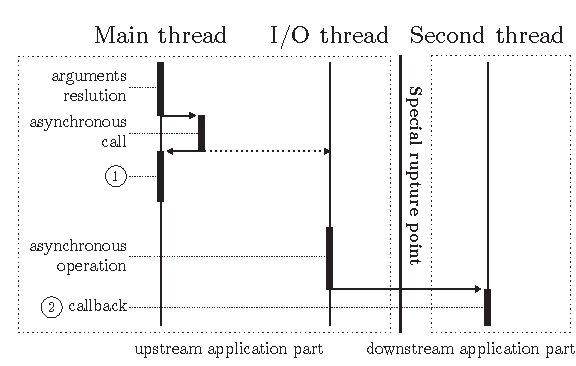
\includegraphics[width=\linewidth]{ressources/specialrp.pdf}
  \caption{Special rupture point interface. \textnormal{The rupture point interface is placed before the asynchronous operation, to avoid moving the result accross the interface from one application part to the other. However, the resolution of the arguments for this asynchronous call is kept upstream to reduce the impact on the application structure}}
  \label{fig:specialrp}
\end{center}
\end{figure}

The application in listing \ref{lst:rupturepoints} presents the two types of rupture points.
The division of this application is illustrated figure \ref{fig:flux-2}.

\begin{code}[js, caption={Example of an application presenting the two types of rupture points. \textnormal{A \texttt{start} with the call to \texttt{app.get()}, and a \texttt{post} with the call to \texttt{fs.readFile()}}},label={lst:rupturepoints}]
var app = require('express')(),
    fs = require('fs');

app.get('/', function handleRequest(req, res) {
  fs.readFile(__filename, function reply(err, data) {
    res.send(err || data.toString());
  })
});

app.listen(8080);
console.log('server listening to 8080');
\end{code}

\begin{figure}[h!]
\begin{center}
  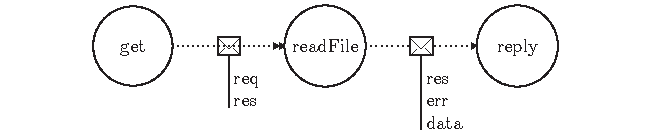
\includegraphics[width=\linewidth]{ressources/flux-2.pdf}
  \caption{Division of the listing \ref{lst:rupturepoints} into three application parts}
  \label{fig:flux-2}
\end{center}
\end{figure}

\subsubsection{Detection}

Detecting a rupture point requires detecting its two components : the asynchronous function and the callback function.

\textbf{Asynchronous functions}\\
The compiler is prebuilt knowing some module names exposing asynchronous functions, like the \textit{express} and the \textit{fs} module in listing \ref{lst:rupturepoints}.
To detect asynchronous calls, the compiler keeps a list of variables holding these modules.
In listing \ref{lst:rupturepoints}, the compiler adds both variables \texttt{app} and \texttt{fs} in this list.
When the compiler encounters a call expression, it compares its callee name with this list to spot asynchronous functions.

\textbf{Callback function}\\
For each asynchronous call detected, the compiler test if one of the arguments is of type \texttt{function} to spot the callback.
Some callback functions are declared \textit{in situ}, and are trivially detected.
For every other variable identifier, we track the declaration up to the initialization value to detect its type.

\textbf{Variable tracking}\\
To detect both the asynchronous function and the callback function, the compiler needs to statically track the types of variables.
Missing rupture points by false negatives in the detection is sub-optimal, but false positives are more critical, as they eventually produce a runtime execution.
Therefore, the detection needs to be as accurate as possible to screen out false positives.
We use a technique similar to a Program Dependency Graph (PDG)\cite{Ferrante1987} to track changes in the value of variables.
This method walks an intermediate representation of the source code to spot the statements modifying a certain variable.
From this intermediate representation, the variable tracker builds a dependency graph which helps the analyzer to detect the type of a variable at a certain point in the execution.
The variable tracker is still in early development and is limited to only a few cases.

\subsection{Linker : memory distribution} \label{section:linker}

\comment{
  As each fluxion is a unique thread accessing a dedicated memory, there is no concurrency, therefor, no synchronization needs, and no possibility of memory corruption.
  But we need to prove that the transformation to message passing is not altering the memory consistency, given the correct isolation.
}

% Because of the central memory, parallelism is not sufficient for an application to be distributed.
Pipeline parallelism is not enough for an application to be distributed.
The compiler also needs to distribute the memory into the application parts for the application to be compliant with the fluxional execution model.
In Javascript, scopes are nested one in the other up to the all-enclosing global scope.
Each function creates a new scope containing variables local to itself, and chained to the scope of the parent function.
% The child function can access variables in the scope of the parent functions, up to the global scope.
Rupture points always take place in between scopes.
A rupture point placed between a child scope and its parent breaks a chain of scopes, and makes the child unable to access its parent as expected, eventually leading the application to a runtime error.
The linker analyzes how scopes are distributed among the application parts to detect and resolve their unmet dependencies.
Depending on how a shared variable is used in the scopes, there are different situations to resolve.
In this section, we explain the different cases of unmet dependencies emerging from the partitioning of a central memory.

\subsubsection{Signature}

The signature is the part of a message containing all the variables to send downstream.
If a variable is needed for read-only access by at least one downstream application part, like the variable \texttt{res} in figure \ref{fig:flux-1}, it is added to the signature of the rupture point.
As fluxions are chained one after another, a fluxion must provide every dependency for the next one, even if some of this dependencies are not needed by the current application part.
These dependencies must be passed fluxion after fluxion from the producing fluxion to the consuming fluxion.
The compiler modifies those variable identifiers inside the application part to make them point to the signature instead of the function scope.

\subsubsection{Scope}

% The scope is the name given to the persisted memory of a fluxion.
The scope of an application part consists of all the variables declared outside, but needed for modification in only this application part.
An example of such a variable is the \texttt{counter} in listing \ref{lst:ex-source}.
Initialized to 0 in the global scope, it is incremented for each request by the \texttt{reply} function.
This counter is in the scope of the application part containing the \texttt{reply} function.
The scope of an application part is stored in the \textit{context} of the encapsulating fluxion.
If one of these variables needs to be read by another application part, this variable also becomes part of the signature sent downstream.

\subsubsection{Sync}

If a variable is needed for modification by more than one application parts, this variable needs to be synchronized between the fluxions.
The synchronization of a distributed memory is a well-known subject, with Brewer's theorem\cite{Gilbert2002}\cite{codahale2010}, and the ACID (Atomicity, Consistency, Isolation, Durability) versus BASE (Basically Available, Soft state, Eventual consistency) opposition\cite{Fox1997}.
We choose to stay out of this topic, the objective for this compiler is to be able to transform only a subset of web applications with a satisfying result.
The compiler merges the parts too tightly coupled by modification accesses on a shared variable.

\subsection{Compilation example} \label{section:example}

% For copyright reason, the compiler source code is kept private along with the tests we used.
To illustrate the compiler features, we compiled the application used as an example for the execution model in section \ref{section:model}.
The source and compiled results of this application are available on github\cite{flx-example}.
The compiler source code is the property of Worldline, and is not publicly available, but we are planning of releasing it as an open source project in the future.

To test the source or the result of the compilation, one would launch respectively \texttt{source.js} or \texttt{result.js} with \texttt{node} and check the service available at \texttt{localhost:8080}.
Both executable needs their dependencies to be resolved with \texttt{npm} before execution.
\begin{verbatim}
git clone https://github.com/etnbrd/flx-example
cd flx-example
npm install
node result.js
open http://localhost:8080
\end{verbatim}

The file \texttt{source.js}, in listing \ref{lst:ex-source}, is the source of this compilation example.
This application sends back its own source along with a download counter.
The processing chain of function is : $\texttt{get} \to \texttt{handler} \to \texttt{readFile} \to \texttt{reply} \to \texttt{send}$.
It uses two asynchronous function call with \textit{in situ} callback, one to listen for user requests and one to read its own source, respectively \texttt{app.get} line 5 and \texttt{fs.read} line 6.
It uses a global variable to increment the download counter defined line 3.
This global variable is used only in the \texttt{reply} function, line 7 and 9.

\includecode{js,
  caption={Source of the compilation example},
  label={lst:ex-source}
}
{../../example/source.js}

The result of the compilation into our high-level language is in the file \texttt{result.flx}, presented in listing \ref{lst:ex-flxres}.
The analyzer detects both asynchronous calls as rupture points.
The first one is a \textit{start} rupture point, associated with the \texttt{app.get} asynchronous function call which makes the callback \texttt{handler} listen for the stream of user requests. 
The second one is a \textit{post} rupture point, associated with the \texttt{fs.readFile} asynchronous function call which reads the source file and hands it to the callback \texttt{reply}.
These two rupture points result in three application parts.
The first application part is encapsulated in the root fluxion, named after the filename, \texttt{source.js}, line 1.
It initializes the system to route the user requests to the fluxion \texttt{handler-1000}, line 8.
This second fluxion reads the file, and sends the result to the next and last fluxion \texttt{reply-1001}, line 14.
We can identify the processing chain of functions in this chain of fluxion.

\begin{center}
\texttt{source.js} (\texttt{get})\\
$\downarrow$\\
\texttt{handler-1000} (\texttt{handler}, \texttt{readFile})\\
$\downarrow$\\
\texttt{reply-1001} (\texttt{reply}, \texttt{send})
\end{center}

The linker detects that the fluxion \texttt{reply-1001} needs two variable to send the result back to the user, \texttt{res} and \texttt{count}.
The variable \texttt{res} depends on the user connection and is initialized for each new request.
It needs to be part of the \textit{signature} of the message transfered to the last fluxion.
The variable \texttt{count} is global, and the \texttt{reply} function in the fluxion \texttt{reply-1001} needs to increment it at each new request.
This global variable is in the \textit{scope} of only this application part, so the compiler stores it in the \textit{context} of this fluxion.
The division by the compiler of this application is illustrated figure \ref{fig:flux-3}.
This result is very similar to the manual division illustrated figure \ref{fig:fluxions}, as expected.

\includecode{flx,
  caption={High level fluxional language result of the compilation example},
  label={lst:ex-flxres}
}
{../../example/result.flx}

\begin{figure}[h!]
\begin{center}
  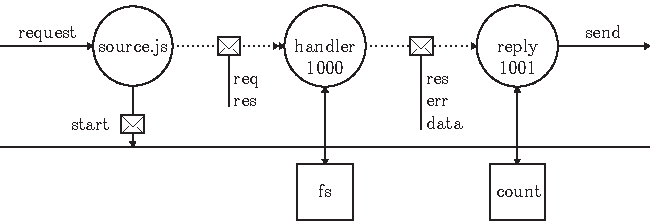
\includegraphics[width=\linewidth]{ressources/flux-3.pdf}
  \caption{Division of the listing \ref{lst:ex-flxres} into three application parts. This result is similar to the manual division illustrated in figure \ref{fig:fluxions}}
  \label{fig:flux-3}
\end{center}
\end{figure}

The compiler also produces an executable targeting a simple implementation of the fluxional execution model.
This result is in the file \texttt{result.js}, presented in listing \ref{lst:ex-jsres}.
The \textit{root} fluxion is not registered because it doesn't need to receive any message by another fluxion, it only initializes the application.
The two following fluxions are registered in the messaging system.
This registration encapsulates the processing function in a \texttt{capsule} function.
The \textit{special rupture points} implies the asynchronous call to be in the downstream fluxion.
The \texttt{capsule} function encapsulates the asynchronous call from a \textit{special rupture points} or the callback from \textit{basic rupture points} in a unified processing function.

The original callback is replaced with a \texttt{placeholder} function, line 3, sending the \textit{start} message to \texttt{handler-1000}.
Line 17, \texttt{handler-1000} pushes the user request \texttt{res} in the message and \texttt{post} it directly to \texttt{reply-1001}.
Because there is a special rupture point between \texttt{handler-1000} and \texttt{reply-1001}, the asynchronous call is moved to \texttt{reply-1001} and the \texttt{post} function doesn't replace the callback, like the placeholder line 3, but is directly called.
Finally, \texttt{reply-1001} receives the message containing the user request and reads the file.
The callback of this asynchronous operation, \textit{reply} function, line 27, increments the variable \texttt{counter}, line 28, and sends the reply, line 30.

\includecode{flx,
  caption={Result of the compilation example targeting the fluxional execution model},
  label={lst:ex-jsres}
}
{../../example/result.js}

\subsection{Limitations}

This compiler aims at transforming a subset of Javascript web applications presenting a specific syntax and design.
In this section, we describe briefly the current limitations of our compiler and how we plan to overcome them in future works.

\begin{itemize}
  \item Variables poorly encapsulated or used too broadly tighten dependencies accross the code, and might result in a coarser division of the application.
  \item The compilation silently fails if a variable holding a callback or a module is overwritten, or not defined in the declaration.
        The variable tracker is unable to track accurately all the modification of a variable to detect these situations which may lead the compiler either to miss rupture points, or to detect non existing one.
  \item The compiler is unable to track a dynamically resolved value, even if the value is deducible statically.
        If this variable is used in a potential rupture point, the compiler screens it out.
  \item The Javascript language offers rich composition possibilities leading to many corner cases.
        The compiler is not robust enough to understand all corner cases.
        For example, the \textit{express} module is only detected if initialized like in listing \ref{lst:rupturepoints}.
\end{itemize}
There may be other limitations we aren't aware of.

The three last limitations described above are caused by the variable tracker - described in section \ref{section:analyzer} - being in an early stage of development.
We are currently in the process of improving the robustness of the compiler to extend the subset of compilable applications.

% We believe that our work will keep scalability concerns out of the way for the development team, who could then focus on the core logic of their application.
% In future developments of this project, we aim at making application dynamically reactive to the load of user requests.
% By monitoring only the input stream, the \texttt{start} rupture points, we believe it is possible to infer the load propagation through the application.
% Using analogy with fluid dynamics, each fluxion is like a pipe, traversed by a fluid of user requests.
% The input and output throughput of this pipe could be calibrated before production use, generating an approximative model of the application reaction to input load.
% Using this model, we want to make the application's reorganize itself in a cluster to handle pikes in the user request throughput.
